\chapter{Scientific Programming} \label{chp:scientificprogramming}
\epigraph{Always code as if the guy who ends up maintaining your code will be a violent psychopath who knows where you live.}{John F. Woods, \cite{woods_usage_nodate}}
\begin{figure}[H]
	\centering
	\copyrightbox[l]{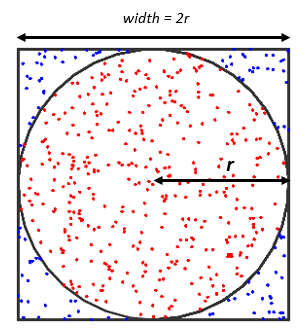
\includegraphics[scale=0.9]{Images/montecarlointegration.png}}{© Copyright 101computing.net}
	\caption{One can estimate the value of $\pi$ using Monte-Carlo integration. Here we approximate the ratio between the area of the circle and the area of the square by counting the number of random points occurring inside the circle and inside the square. The estimate of $\pi$ is found from $\pi=4\cdot A_{\text{circle}}/A_{\text{square}}$.}
	\label{fig:montecarlointegration}
\end{figure}

Since this scientific work is based on solving equations numerically on the computer, software development is a major part of the work. We will in this chapter go through the main concepts of scientific programming, and directly relate them to our code in the next chapters on implementation. As a motivation, we will provide a brief recap of some historical milestones in scientific computing.

Computers have long been used for solving complex scientific problems. Actually, for a long time science was the main motivation of developing computers. Already in 1929, Egil Hylleraas used his mechanical desk calculator to calculate the ground state energy of the Helium atom, which remains a milestone in computational quantum chemistry as well as quantum chemistry in general \cite{helgaker_perspective_2000}. Later, pioneers like Alan Turing and John von Neumann contributed to the invention of the first electronic computer, which made numerical solutions of ordinary differential equations possible \cite{gustafsson_scientific_2018}. 

Also on the software side, big breakthroughs have been made since the advent of the electronic computer. The programming language Fortran was released in 1957, which provided a new basis of scientific programming \cite{allen_history_1981}. Later, Ole Johan Dahl and Kristen Nygaard developed the language SIMULA, which is considered as the first object orientated language \cite{holmevik_compiling_1994}. The language that we mostly will rely on in this work, C++, is an extension of the language C which was developed in the early 1970's and is, together with Fortran, one of few languages that have survived the ravages of time. 

The computers used today, included both the hardware and the software, have become possible due to heroic effort of an array of scientists, engineers and mechanics over a long period. The computers are stronger than ever, have more memory than ever, are compacter than ever and, last but not least, they are more user-friendly than ever. This has made heavy computations that was unthinkable just decades ago possible, and has contributed to the development of essentially all branches of science. Due to the user-friendliness, advanced simulations have also been available to young and curious students like the author, which we should not take for granted. 

The computer's language itself is binary, and is the lowest level. To translate commands to this language, we need a "translator", which is a language that fills the gap between the binary language and human commands. This language is categorized in levels based on how similar they are to the binary language. Low-level languages are more similar to the binary language than a high-level language. The result is that low-level languages in general are more demanding to deal with, but they are typically faster than high-level languages. In our work, we have used the low-level language C++ for the main code, but for scripting, including plotting and solving less expensive problems, the high-level language Python has been used. 

In this chapter, we will explain the essentials behind scientific programming, using examples from both C++ and Python. We will begin from the very basic, so if the reader is an experienced programmer this chapter will probably be perceived as old news. Programs are often either classified as \textit{procedural programming} or \textit{object oriented programming}, based on whether the code is written in the same order as the program flow goes (procedural) or is based on objects (object-orientated).

\section{Object orientated programming in Python}
In the everyday life, we are surrounded by objects all the time which can be placed in different categories. For instance, a \textit{circle} is an object with properties like area, circumference and so on, and can be placed in the class \textit{shapes}. Other members of the class shapes might be square and triangle. In object orientated programming, we create similar objects, or classes, to make the program flow more intuitive for the reader. The main class is called the parent class, while the sub-classes are called the children. The reason for this analogy, is that the sub-classes always inherit from their main class, but not the other way around. 

The example with the shapes can therefore be implemented with \texttt{Shapes} being the parent, and \texttt{Circle}, \texttt{Square} and \texttt{Triangle} being its children. In the high-level language Python, this can be implemented as 

\lstset{basicstyle=\scriptsize}
\begin{lstlisting}[language=python]
import numpy as np

class Shapes:
	def __init__(self, r):
		self.r = r

	def getArea(self):
		raise NotImplementedError("Class {} has no instance 'getArea'."
				.format(self.__class__.__name__))


class Circle(Shapes):
	def getArea(self):
		return np.pi*self.r**2

	def getCircumference(self):
		return 2*np.pi*self.r

	def getExtent(self, x, y):
		if np.linalg.norm([x,y]) < self.r:
			return True
		return False

class Square(Shapes):
	def getArea(self):
		return 4*self.r**2

	def getCircumference(self):
		return 8*self.r

	def getExtent(self, x, y):
		if abs(x) < self.r and abs(y) < self.r:
			return True
		return False

class Triangle(Shapes):
	def getCircumference(self):
		return 6*self.r
\end{lstlisting}
where we give the children the properties area, circumference and extent. The length \texttt{r} means the radius of a circle, half the side length of a square and also half a side length of the equilateral triangle, see figure \eqref{fig:montecarlointegration}. We can implement a circle, square and triangle of \texttt{r}=1, respectively named "circ", "squr" and "tria" by these three lines
\lstset{basicstyle=\scriptsize}
\begin{lstlisting}[language=python]
circ = Circle(1)
squr = Square(1)
tria = Triangle(1)
\end{lstlisting}
Moreover, we can easily get their areas by calling the \texttt{getArea()} function,
\lstset{basicstyle=\scriptsize}
\begin{lstlisting}
>>> circ.getArea()
3.141592653589793

>>> squr.getArea()
4

>>> tria.getArea()
NotImplementedError: Class Triangle has no instance 'getArea'.
\end{lstlisting}

As we can see, the area of the circle and the square were calculated successfully, giving $\pi r^2$ and $4r$ respectively. On the other hand, the area of the triangle raised an error, which is obviously because we do not have defined the area of the triangle! This example illustrates that properties of the children overwrites the properties of the parent, but if the children does not have the called property, it will instead return the parent's property. 

\subsection{An example based on Monte-Carlo simulations}
Up to this point, we have talked a lot about Monte-Carlo simulations without giving an illustrating example on what it is. Methods where we draw numbers randomly from a function to reveal properties of the function are in general categorized as Monte-Carlo simulations. 

Suppose we did not know the value of $\pi$, what could we do to approximate its value? There are many ways to do this, where the most intuitive might be to measure the ratio between the diameter and the circumference in a circle. It is not possible to do this very accurate manually. A more accurate and robust solution would be to use Monte-Carlo simulations, where we for instance can take the starting point on the relation
\begin{equation}
\pi=4\frac{\text{A}_{\text{circle}}}{\text{A}_{\text{square}}}
\end{equation}
which is derived from the ratio between the circle area and the square area. By drawing random numbers from a uniform distribution and count the number of points which are in the square and in the circle, we can approximate $\text{A}_{\text{circle}}/\text{A}_{\text{square}}$. We can do this by using the \texttt{getExtent()} function of the square class and circle class,
\lstset{basicstyle=\scriptsize}
\begin{lstlisting}[language=python]
for i in range(1,10):					# Iteration loop
	M = 10**i
	A_square = 0
	A_circle = 0
	for _ in range(int(M)):				# Monte-Carlo loop
		x = np.random.uniform(-1,1)
		y = np.random.uniform(-1,1)
		if circ.getExtent(x,y):
			A_circle += 1
		if squr.getExtent(x,y):
			A_square += 1
	print("Pi: ", 4 * A_circle/A_square)
\end{lstlisting}
which gives a output similar to
\begin{lstlisting}
Pi:  2.4
Pi:  3.32
Pi:  3.156
Pi:  3.1296
Pi:  3.14168
Pi:  3.140044
Pi:  3.1420708
Pi:  3.1416844
Pi:  3.141615628
\end{lstlisting}
Considering the fact that $\pi=3.141592653589793...$, the obtained result is quite acceptable. However, to run the program with $M=10^9$ Monte-Carlo cycles, the program is quite slow. Is it possible to do this faster? The answer is yes, by switching entirely or partly to a low-level language.

\section{Low-level programming with C++}
Above, we looked at how inheritance can be implemented in the high-level language Python, and we observed the main weakness of high-level languages: the computational time. In this section, we will repeat the implementation and example above using C++. This will, hopefully, provide a significant speed-up. A similar class structure in C++ looks like
\lstset{basicstyle=\scriptsize}
\begin{lstlisting}[language=c++]
class Shapes {
	public:
		Shapes();
		virtual double getArea() = 0;
		virtual double getCircumference() = 0;
		virtual bool getExtent(double x, double y) = 0;
		virtual ~Shapes();
};

class Circle : public Shapes {
	public:
		Circle(double r);
		double getArea() {
			return M_PI * m_r * m_r;
		}
		double getCircumference() {
			return 2 * M_PI * m_r;
		}
		bool getExtent(double x, double y) {
			if(sqrt(x*x+y*y) < m_r) {
				return true;
			}
			return false;
		}
	private:
		double m_r = 1;
};

Circle::Circle(double r) : Shapes() {
	m_r = r;
}

class Square: public Shapes {
	public:
		Square(double r);
		double getArea() {
			return 4 * m_r * m_r;
		}
		double getCircumference() {
			return 8 * m_r;
		}
		bool getExtent(double x, double y) {
			if(fabs(x) < m_r && fabs(y) < m_r) {
				return true;
			}
			return false;
		}
	private:
		double m_r = 1;
};
Square::Square(double r) : Shapes() {
m_r = r;
}
\end{lstlisting}
which looks quite different from the implementation in Python. We will go thoroughly through the different part of the code. 

One of the first thing we observe, is that we here need to \textit{declare} all the variables, which means that we need to specify what kind of variable it is. In the following we will have a look at some standard \textit{data types}.

\subsection{Built-in data types}
In low-level languages we need to specify the data types manually, giving us more control and flexibility. The most fundamental data types are \texttt{int} representing an integer number, \texttt{float} representing a floating number, \texttt{bool} representing a Boolean number and a \texttt{char} representing a character.

Often, these four data types are not sufficient for the task we want to implement and we need to introduce more data types. An especially common error is \textit{overflow}, meaning that the number computed is out of the range of our data type. To avoid this, we can switch to data types of longer range, replacing \texttt{int} with a \texttt{long long int} (or just a \texttt{long long}), and replacing \texttt{float} with a \texttt{double}. 

Some languages also deal with \texttt{long int} and \texttt{long double}, but in C++ an \texttt{int} and a \texttt{long int} is the same. Additionally, a \texttt{long double} is the same as a \texttt{double}. As lack of memory seldomly is a problem on modern computers, it is common to declare all floating numbers as \texttt{double}s. In table \eqref{tab:datatypes}, the most common data types are listed with their range and memory occupation in C++.

\begin{table}
	\caption{Built-in data types in C++, with their memory occupation and range. Parenthesis () means that the the extension is optional. Numbers are taken from \cite{noauthor_c++_2017}.}
	\label{tab:datatypes}
	\begin{tabularx}{\textwidth}{R{0.5cm}L{7cm}R{1.5cm}R{5cm}R{0.3cm}} \hline\hline
		&\makecell{\\ Data types \\ \phantom{=}} & Size [bytes] & Range & \\ \hline \\
		&(\texttt{signed}) \texttt{short} (\texttt{int}) & 2 & $-2^{15}$ to $2^{15}-1$ & \\
		&(\texttt{signed}) \texttt{int} / \texttt{long} (\texttt{int}) & 4 & $-2^{31}$ to $2^{31}-1$ & \\ 
		&(\texttt{signed}) \texttt{long long} (\texttt{int}) & 8 & $-2^{63}$ to $2^{63}-1$ & \\
		&\texttt{unsigned short} (\texttt{int}) & 2 & 0 to $2^{16}$ & \\
		&\texttt{unsigned int} / \texttt{unsigned long} (\texttt{int}) & 4 & 0 to $2^{32}$ & \\ 
		&\texttt{unsigned long long} (\texttt{int}) & 8 & 0 to $2^{64}$ & \\
		&\texttt{float} & 4 & $\sim$ $\pm$3.4E38 ($\sim$ 7 digits) & \\
		&(\texttt{long}) \texttt{double} & 8 & $\sim$ $\pm$1.7E308 ($\sim$ 15 digits) & \\
		&(\texttt{signed}) \texttt{char} & 1 & $-2^7$ to $2^{7}-1$ & \\ 
		&\texttt{unsigned char} & 1 & 0 to $2^{8}$ & \\ 
		\hline\hline
	\end{tabularx}
\end{table} 

For integers it is also possible to "move" the range from its zero-centered default to only include positive numbers. This is done by declaring a \texttt{unsigned int} or \texttt{unsigned long}. This doubles the range in the positive direction, but should not be done if one, by any chance, can get negative numbers, as one will get \textit{underflow}.  

\subsection{Access modifiers}
Another thing that we observe from the code example above, is that we define the functions as \texttt{private} or \texttt{public}, which are called access modifiers. The access modifiers specify how much access the environment should have to the function: \texttt{private} means that the function can only be called from the particular class, while \texttt{public} means that also sub-classes (children) and other classes have access to the function. 

We also have a third access modifier in C++, called \texttt{protected}. \texttt{protected} members of a class A are not accessible outside of A's code, but any class that inherit from A has access to the protected member. 

\subsection{Pure virtual functions}
In Python, we saw how a parent's function was overwritten by a function of the child. This work as long as the child's function has identical name and identical arguments as the parent's function, otherwise it all will fail.

In C++, a much safer method exists based on pure virtual functions, where a child is \textit{forced} to have the same virtual functions as its parent. The virtual functions of the parent therefore serves as a template of its children, such that all the children have the same features. 

This is often very useful, as the children tend to have the same features. Taking it back to the \texttt{Shapes} class, all the shapes ought to have features area and circumference, which can be forced by using virtual functions, as done in the example above. 

\subsection{Constructors and destructors}
In the example above, we observe that the class \texttt{Shapes} has a function with the same name, \texttt{Shapes} and another virtual function $\sim$\texttt{Shapes}. The former one is used to create the object, and is hence named a \textit{constructor}. This function gets called automatically when the object of a class is created. Similarly, the latter one destructs an object when we are done evaluating the object. It is therefore named a \textit{destructor}, and is also called automatically when an object is deleted or goes out of scope.

\subsection{Pointers}
In the example above, we have not directly used any pointer. However, pointers are important in low-level languages, and we will here give a very brief introduction to pointers.

For a C++ program, the memory of a computer is like a succession of memory cells, each with a unique address and of size one byte. When declaring a variable of size larger than one byte, the object will occupy memory cells that have consecutive addresses. Often, it is useful to know this address, which allows you to change the object directly in the memory. The address of a variable is given by the address-of operator, \&, working as
\lstset{basicstyle=\scriptsize}
\begin{lstlisting}[language=C++]
address=&variable
\end{lstlisting}
Doing this, we say that we \textit{point to the address}, and a variable that stores the address of another variable is thereby called a pointer. 

Furthermore, the dereference operator, *, gives the value of the address to where a pointer points. Thus, the following is true
\begin{lstlisting}[language=C++]
variable=*address
\end{lstlisting}

\subsection{Back to the Monte-Carlo example}
We can now call the class above from the \texttt{main} function. We start defining the children \texttt{circ} and \texttt{squr}, and use the \texttt{getExtent()} function to approximate the area ratio between them. The code looks like 
\begin{lstlisting}[language=c++]
int main() {   
	class Shapes* circ = new Circle(1);
	class Shapes* squr = new Square(1);

	for(int i=1; i<10; i++) {
		int M = int(pow(10,i));
		long A_square = 0;
		long A_circle = 0;
		for(int m=0; i<M; i++) {
			double x = uniform(gen);
			double y = uniform(gen);
			if(circ->getExtent(x, y)) {
				A_circle ++;
			}
			if(squr->getExtent(x, y)) {
				A_square ++;
			}
		}
		std::cout << std::fixed;
		std::cout << std::setprecision(10);
		std::cout << "Pi: " << 4 * double(A_circle)/A_square << std::endl;
	}
	return 0;
}
\end{lstlisting}
which gives the same output as the Python script, but is much faster. 

\iffalse
\subsection{Data types in Eigen}
The open source template library for linear algebra, Eigen, will be used throughout the coding, and it comes with arrays of various properties. The most relevant ones are \texttt{VectorXi}, which has dynamic length and \texttt{int} data type and \texttt{VectorXd}, which has dynamic length and \texttt{double} data type. The Matrix class has equivalent objects. 

In cases where we have \textit{a priori} knowledge of the array size, we can replace the \texttt{X} with the actual size. A fixed $3\times 3$ matrix of type \texttt{double} can for example be declared as \texttt{Matrix3d}. According to the Eigen documentation, using fixed size is \textit{"...hugely beneficial to performance"}. \url{https://eigen.tuxfamily.org/dox/group__TutorialMatrixClass.html}.
\fi